\section{Exercise two}

Describe (the answer has to be effectively supported) a 1-BHT and a 2-BHT able to execute the following assembly code (R0 is set to 1, R1 is set to 300). 
\begin{verbnobox}[\verbarg]
LOOP:   LD F3 0 (R0)
        ADDD F1 F3 F3
        ADDI R1 R1 3000
LOOP2:  MULTD F2 F2 F3
        SUBI R1 R1 3
        BNEZ R1 LOOP2
        SUBI R0 R0 2
        BNEZ R0 LOOP
\end{verbnobox}
The obtained result, in terms of mispredictions, is inline with theoretical characteristics of the two predictors? 
Please effectively support your answer.

\subsection*{Solution}
We have that $R0$ is set to 1, and $R1$ is set to 300. 
The internal loop is looped $\frac{3300}{3}=1100$ times. 
The register for the external loop becomes $-1$ before the first branch check, and so we have an infinite loop (impossible to have $R0$ set to zero)

For the one-bit branch table computation, a finite state machine can be employed, depicted below:
\begin{figure}[H]
    \centering
    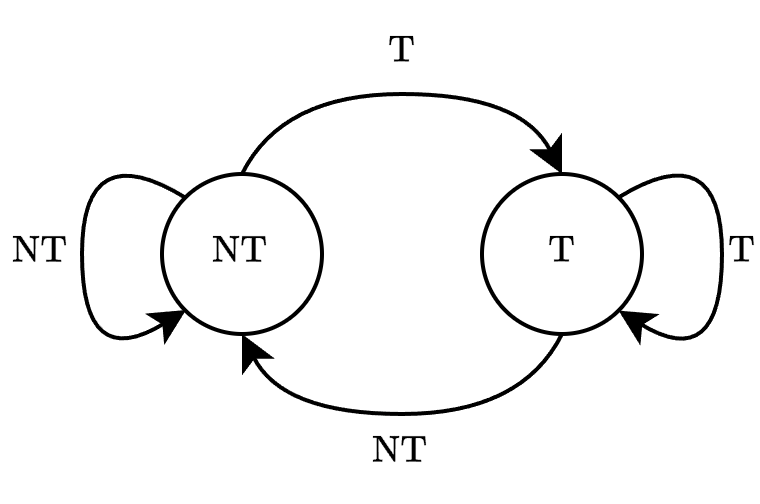
\includegraphics[width=0.4\linewidth]{images/1bht.png}
\end{figure}

In the absence of collision, one bit can be assigned for each loop. 
This allows four possible initializations: T-T, T-NT, NT-T, NT-NT.
\begin{itemize}
    \item For the first case (T-T), there are NO misprediction for loop, and for loop2 a single misprediction at the end of the loop @T0 + 2 misprediction x iteration begin and end of the loop
    \item For the second case (T-NT), there are NO misprediction for loop, and for loop2 two misprection: beginning and end of the loop
    \item For the third case (NT-T), there are only initial misprediction for loop, and for loop2 single misprediction at the end of the loop @T0 + 2 misprediction x iteration begin and end of the loop
    \item For the fourth case (NT-NT), there are only initial misprediction for loop, and for loop2 two misprection: beginning and end of the loop. 
\end{itemize}

In the presence of collision, one bit is allocated for each loop. 
This yields two possible initializations: T, NT.\@
The iterations for each case are calculated as follows:
\begin{itemize}
    \item For the first case (T), there are  single misprediction at the end of the loop2, and a 100\% failure rate for loop. 
    \item For the second case (NT), there are two initial misprection, then end of the loop and a 100\% failure rate for loop. 
\end{itemize}

The two-bit branch table can be designed using a finite state machine, as illustrated below:
\begin{figure}[H]
    \centering
    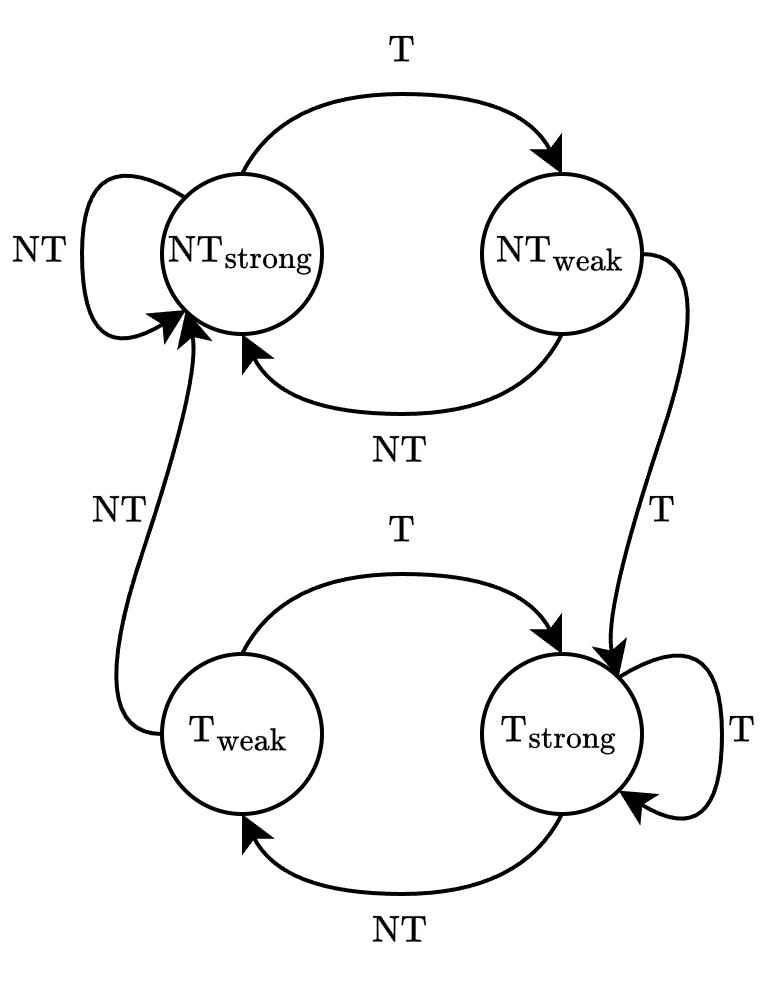
\includegraphics[width=0.4\linewidth]{images/2bht.png}
\end{figure}
In the absence of collision, where one bit is assigned for each loop, there are eight possible initializations.
The worst cases are:
\begin{itemize}
    \item $\text{NT}_{\text{weak}},\text{NT}_{\text{weak}}$: resulting in $2\times\infty$ mispredictions for LOOP2 and $1$ mispredictions for LOOP.\@
    \item $\text{NT}_{\text{strong}},\text{NT}_{\text{strong}}$: resulting in $2+1+1\times\infty$ mispredictions for LOOP2 and $2$ mispredictions for LOOP.\@
\end{itemize}
The best cases are: 
\begin{itemize}
    \item $\text{T}_{\text{weak}},\text{T}_{\text{weak}}$: Resulting in $1 + 2\times\infty$ mispredictions for LOOP2 and $0$ for LOOP.\@
    \item $\text{T}_{\text{strong}},\text{T}_{\text{strong}}$: Resulting in $1 \times\infty$ mispredictions for LOOP2 and $0$ for LOOP.\@
\end{itemize}